\chapter{Question-Asking and Plan Inference}
\label{ch:question_plan}
\textbf{Salena Ashton, Stephen Kim, Loren Rieffer-Champlin, Liang Zhang,
Adarsh Pyarelal, Clayton Morrison}

\section{Introduction}

As people interact with each other, they display observable behaviors (speech,
body language, expressed emotion, or interaction with the environment) that may
suggest unobservable behaviors (thoughts, feelings, plans, or beliefs). The
process of inferring these unobservable behaviors is called \emph{theory of
mind} (ToM) and is often studied through the analysis of body language, spoken
natural language, human development, social cultural differences or
non-neurotypical human cognition. When humans ask questions to obtain
information, they most likely do so with an intent, a plan, or desire.

Within AI, a \emph{classical plan}, also called flat, is a sequence of states
and simple actions that an agent can execute to reach a goal. These plans can
be represented with a flat data structure such as a list. As plans become more
complex, require constraints, or have multiple levels of abstraction within the
same plan, they are best represented by a \emph{hierarchical task network}
(HTN), which is a tree of possible plans.\footnote{Technically, the plans
    produced by HTN planners can also be represented with flat lists - however,
in this section, we use the term `plan' to refer to the actual `plan tree' that
contains the task decompositions as well, rather than just the plan alone.}

We will investigate the following hypotheses for Study-3:

\begin{enumerate}

    \item How do spoken questions reveal another person’s plan or intent? We
        will investigate whether verbalized question-asking can infer a human’s
        ToM when uttered in a simulated search-and-rescue (SAR) scenario within
        the Minecraft environment, as designed by ASIST.

    \item Can those who listen to these questions accurately decide if the plan
        is simple, sequential, or hierarchical? The results of this
        investigation will guide further research about how to infer and best
        represent a human's plans as either flat or corresponding to a
        hierarchical task decomposition. Can the distinction between such
        structures improve predictive performance for Artifical Social
        Intelligence (ASI) agent intervention?

\end{enumerate}


Existing literature about HTNs, ToM, psycholinguistics and question-answering
are abundant, as are papers about question generation for information
retrieval. Few papers focus on the intersection of ToM for human beings and the
HTN mapping of dialog acts. \citet{hawkins_goodman_2017}
approach question-asking as evidence of the questioner’s hidden goals. They
categorize questions into binary question-answer pairs, pragmatic
question-answer pairs where the most socially-acceptable response does not
strictly answer the literal question asked, and probabilistic question-answer
pairs, where the most probable answer is the expected value of a set of likely
answers. Within the SAR scenario of ASIST’s Minecraft environment, human
players will verbalize plans, suggestions, or ideas to each other. Sometimes
these plans or requests are fulfilled and other times they are violated,
forgotten or disregarded. \citet{DBLP:conf/atal/BaldoniBCM19} discuss social
interactions of AI agents with first-order logic; this representation includes
question-asking and the life cycle of agent commitments. This representation
can also express action sequence and constraints of actions and plans.

\section{Approach}

We assume that questions have hidden goals and infer plans. As teams ask more
questions of each other, human team ToM converges toward cooperative behavior.
We will investigate whether question-asking is associated with \emph{team
planning}, defined as a set of goals, strategies, or tasks that are executed.
We define \emph{coordination} as behaviors and utterances to create a common
plan or strategy\footnote{Note that this is distinct from the mathematical
definition of coordination proposed in \autoref{ch:pgm}}. We define
\emph{cooperation} as team behaviors that implement an already-agreed up on
plan.

To capture hidden goals, inferred plans, and patterns that may represent human
ToM, we will annotate six ASIST Study 3 Spiral 2 pilot video observations and
six HSR ASIST Study 3 videos released between March 29 and May 5, for a total
of at least twelve videos. These videos are of three distinct missions for each
team. Due to the expensive costs of taxonomy label development with strict
adherence to grounded theory methodology, this stage of the experiment is
limited to no less than twelve videos. 

Two human annotators will code all uttered questions between teammates within the Minecraft SAR scenario.
We use the qualitative coding procedure known as Grounded Theory,
as defined by \citet{corbin_strauss_2015}. 

More specifically, and as defined by \citet{saldana_2021}, we will use a
Grounded Theory Process Coding for a state or action across some interval of
time. These \emph{grounded-in-data} labels are known as \emph{concept-level}
labels, which are the smallest pieces of data that encode a question-asking
phenomena of interest.

We will use a Grounded Theory Causal Coding to investigate the connectivity and
causality of each concept label to discover possible relationships between
presence or absence of team actions, interactions, conditions, and consequences
of question-asking. Densely-connected concept labels suggest subcategories and
categories. Sparsely-connected labels will not be discarded; they will be used
to consider variability within patterns and categories that emerge. In cases
where questions have co-reference or other contextual dependencies, only that
direct dependency will be coded for local semantic meaning.

We make the following considerations when creating codes: 

\begin{itemize}
    \item Frequency will not dictate importance, causality, or connectivity of a concept
    \item Each question will have at least one annotation and up to four
      annotations:
    \begin{itemize}
        \item Primitive actions (ground truth). Ex: breakRubble,
          requestStabilizedVictimCarry.
        \item Abstraction Levels of actions (of primitive actions) Respective
          examples: respondRubbleRequest or createVictimAccess, collaborateStabilizedVictim
    \end{itemize}
    \item Labels will be stemmed and minimally normalized
    \item Capturing the phenomena of question-asking across time, between any subset of a team, between the same team across the two different missions. 
\end{itemize}


To avoid annotator and researcher biases and any \emph{a priori} belief on
which team ToM strategies may be used, concept and category labels are not
pre-determined. Inter-annotator agreement must reach a Kappa Score of 80\% or
higher. This also gives a more solid, grounded analytical meaning to any
emergent categories. 

After the development of labels and taxonomy, the investigation of team ToM and
question-asking will scale for additional videos. When all concepts,
subcategories, categories can reasonably explain the phenomena of the video
observations, one or two super-categories, \emph{theories of team plan}, will
emerge. We currently assume that a theory of team plan would have greater
predictive power and ToM inference potential. 


\section{Evaluation}

Because of the small sample size of this investigation, we will not perform a
quantitative evaluation at this time. Instead, we will perform a qualitative
investigation of word frequencies, clustering patterns, and correlation of
annotator-generated labels through data visualization. Below is a list of
possible visualizations we may consider:

\begin{itemize}

    \item Connectivity of concept-level labels: radial diagrams, arc diagrams,
        matrix diagrams or graph networks

    \item Frequency patterns of words or concept labels (normalized, word count
        / total number of words in that question): scatterplots or histograms

    \item Correlation of words and labels with time: time series, scatterplots. 

    \item Concept-level subcategorization(s): clustering, PCA (concept labels
        possibly projected onto sub-categorical spaces), or hierarchical
        visualizations.

\end{itemize}


These visualizations serve as a preliminary analysis of how uttered
questions, with their hidden goals, could map human ToM to AI planning data
structures. Tthe following visualization shows the distribution of
qustions asked across time for two pilot study teams. 


\begin{figure}[h]
    \centering
    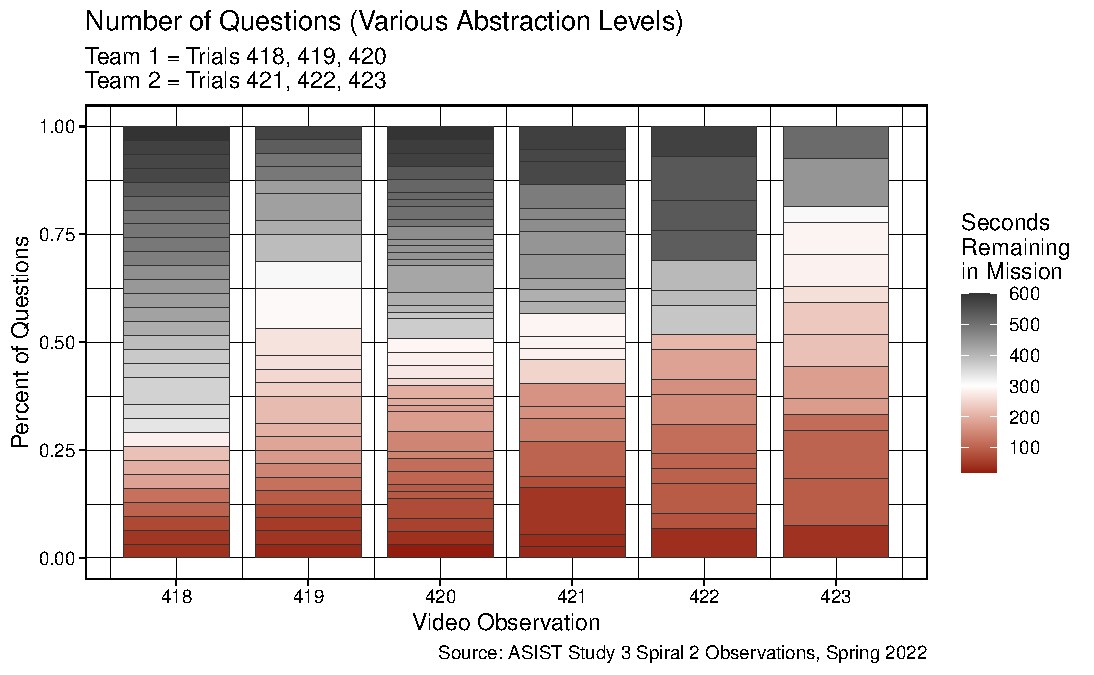
\includegraphics[width=0.9\textwidth]{images/prelim_percent_questions.pdf}
    \caption{Questions asked during three missions of two distinct teams across
    time. Black indicates questions asked toward the beginning of each mission
  and red indicates questions asked toward the end of each mission. This 
suggests that teams ask more questions toward the beginning of the
first mission and the end of the last mission.}
\end{figure}


Such visualizations, based on twelve videos, will lead to further insight
through this investigation. Future measures may include Mann-Whitney U-Tests,
t-tests (only if we annotate a large-enough sample), precision and recall of
the concept-level and category patterns to describe the generalizability for
real data with no ASI interventions, generalizability for real data with ASI
interventions, and the variance of patterns in label categories. Another
possible measure, for future research, would be the F1 score to explain how
well these labels describe observations without ASI interventions, when
compared to high-intervention observations. This future investigation would
address measure ASI-M5: Coordinative Communications to
measure teamwork, include additional video observations for real data in Study
3, and continue our investigation of whether human plans and ToM are best
represented by classical planning or HTN planning.


